\documentclass[10pt,twocolumn,letterpaper]{article}
\usepackage[T1]{fontenc}
\usepackage[utf8]{inputenc}
\usepackage{times}
\renewcommand{\ttdefault}{cmtt}
\renewcommand{\sfdefault}{cmss}
\usepackage[margin=0.72in,columnsep=0.26in]{geometry}
\usepackage{graphicx,booktabs,array,tabularx}
\usepackage[round,authoryear]{natbib}
\usepackage[colorlinks=true,allcolors=black,breaklinks=true]{hyperref}
\usepackage{url}
\urlstyle{same}
\makeatletter
\newenvironment{staticfigure}{\par\medskip\noindent\begin{minipage}{\linewidth}\def\@captype{figure}}{\end{minipage}\par\medskip}
\newenvironment{statictable}{\par\medskip\noindent\begin{minipage}{\linewidth}\def\@captype{table}}{\end{minipage}\par\medskip}
\makeatother
\setlength{\parindent}{1em}
\setlength{\parskip}{0pt}
\setlength{\textfloatsep}{12pt plus 2pt minus 2pt}
\setlength{\floatsep}{10pt plus 2pt minus 2pt}
\setlength{\dbltextfloatsep}{13pt plus 2pt minus 2pt}
\setlength{\abovecaptionskip}{5pt}
\setlength{\belowcaptionskip}{3pt}
\renewcommand{\topfraction}{0.88}
\renewcommand{\bottomfraction}{0.75}
\renewcommand{\textfraction}{0.10}
\renewcommand{\dbltopfraction}{0.88}
\setcounter{topnumber}{4}
\setcounter{dbltopnumber}{4}
\emergencystretch=2em
\raggedbottom
\date{}
\hypersetup{pdftitle={Task Success and Written Reasoning in Sokoban Reinforcement Learning},pdfauthor={Yihao Tao, Bowu, Jintao Wang, Runhu, Haotian Liu}}
\title{\LARGE\bfseries Task Success and Written Reasoning in Sokoban Reinforcement Learning}
\author{Yihao Tao \quad Bowu \quad Jintao Wang\\[3pt]Runhu \quad Haotian Liu}
\begin{document}
\twocolumn[\begin{@twocolumnfalse}
\maketitle
\vspace{-1.9em}
\begin{abstract}
An agent can become better at a task while producing less informative explanations of its actions. We examine this separation in a small reproduction and extension of RAGEN using Qwen2.5-0.5B-Instruct on text-based Sokoban. Eight models are trained for 200 updates with reward-variance filtering, random group selection, an ineffective-action penalty, or no filtering. On 512 fixed test environment seeds, StarPO-S reaches 21.94\% mean success across three training seeds, compared with 4.36\% for random selection. In the first StarPO-S run, validation success rises from 5.08\% to 21.09\%, while mean thought length falls from 25.07 to 3.79 words and exact think-answer agreement rises from 1.12\% to 97.62\%. The two additional StarPO-S runs exhibit the same final output pattern. Two comparison runs produce no executable actions at the final checkpoint; an action penalty improves one test score but increases the fraction of ineffective moves. We audit repeated initial boards and obtain the same method ordering after excluding validation-board matches. These results support separate measurement of task performance, training stability, and written reasoning, without treating generated explanations as direct evidence of internal computation.
\end{abstract}
\vspace{1em}
\end{@twocolumnfalse}]
\section{Introduction}\label{sec:intro}
When a language model acts in an environment, its written explanation and its executed action can improve at different rates. A valid action may move a box closer to a target even if the accompanying explanation merely repeats the action name. Conversely, fluent text may describe a board incorrectly and lead to a failed episode. Evaluating only task reward leaves this distinction unresolved.

RAGEN provides a framework for studying such behavior through multi-turn reinforcement learning. Its StarPO formulation optimizes interaction trajectories, and StarPO-S combines reward-variance filtering with a critic and asymmetric clipping to stabilize training \citep{ragen}. The original study also reports that task-oriented rewards need not sustain detailed written reasoning. We investigate these issues in a smaller, single-environment setting where training records and individual action sequences can be inspected directly.

Our central comparison changes which state groups contribute to each policy update. Selecting the groups with the largest variation in trajectory reward is compared with selecting the same number of groups randomly. This separates the selection criterion from the number of retained episodes, although generated token counts and elapsed computation remain unconstrained. Two additional runs examine an ineffective-action penalty and training on all sampled trajectories.

We find a consistent descriptive advantage for variance-based selection across the three tested training seeds. Yet the successful runs increasingly emit the same short action list in both the thought and answer fields. Thus, maintaining useful task behavior does not by itself maintain a verbal account of the board or plan. Our evidence comprises all eight final models, checkpoint-level text statistics, and failure diagnostics. The source, configurations, raw trajectories, and analysis code are publicly available \footnote{\url{https://github.com/Kris-Liu773/ragen-sokoban-reproduction}}. This is an empirical study of an existing method, rather than a new optimization algorithm or a reproduction of every RAGEN experiment.

\section{Experimental Design}\label{sec:design}
\subsection{Environment and interaction protocol}
We use SimpleSokoban: a 6 by 6 text grid containing one player, one box, and one target. The player can move up, down, left, or right and can push a box but cannot pull it. An episode succeeds when the box reaches the target. The agent receives the current grid, the remaining action budget, and prior interaction history. It is prompted to return a \texttt{<think>} span followed by an \texttt{<answer>} span containing actions separated by \texttt{||}. The parser can execute up to five actions from a turn. Episodes stop after success, five model turns, or ten executed actions.

The generator allows up to 400 new tokens per turn; the inherited prompt separately requests a 100-word/token response. Training samples at temperature 1.0 and evaluation at 0.5. All variants use the original environment return and the inherited format penalty of -0.1 for a turn with missing or invalid actions. No reward directly scores the factual accuracy or usefulness of the thought text. The additional ineffective-action penalty described below is distinct from this shared format penalty.

\subsection{Model and optimization}
The policy is initialized from Qwen2.5-0.5B-Instruct \citep{qwen}. We use the first RAGEN implementation and its veRL training backend \citep{hybridflow}, with full actor and critic fine-tuning. Updates use proximal policy optimization \citep{ppo} and generalized advantage estimation \citep{gae}. The actor and critic learning rates are $10^{-6}$ and $10^{-5}$, respectively. Both the discount factor and GAE parameter are 1.0. The PPO ratio bounds are 0.80 and 1.28, the entropy coefficient is 0.001, and the KL coefficient is zero. Each update performs one PPO epoch with a mini-batch size of 32 and a GPU micro-batch size of four.

The historical configuration optimizes serialized trajectories with \texttt{enable\_response\_mask=false}. Its loss mask includes non-system context as well as assistant segments; we preserve this behavior rather than replace it with assistant-only optimization. Rewards are accumulated at the trajectory level with identity reward normalization. These implementation choices are shared by all variants. Appendix \ref{app:reproduction} records the exact source revisions and other settings.

\subsection{Selection and reward variants}
Every update samples eight initial state groups and generates 16 episodes from each state, for 128 sampled episodes. StarPO-S retains the two groups with the highest within-group sample standard deviation of trajectory scores. All 16 episodes in each retained group are used, including unsuccessful attempts. The result is 32 update episodes, selected for diversity of outcomes rather than for high score alone.

Random selection retains two uniformly sampled groups without replacement, also giving 32 update episodes. Its selection RNG is separate from the environment RNG. The critic, clipping, and remaining optimization settings are unchanged. Consequently, this comparison tests the group-selection rule within the same training setup; it does not remove every stabilization component of StarPO-S.

The penalty variant adds -0.1 for each executed move that leaves the player position unchanged, then applies the standard variance filter. The extra penalty is used only during training. No filter retains all 128 episodes. With mini-batches of 32, it processes four times as many episodes and mini-batches per outer update as the filtered variants. It is therefore a diagnostic comparison, not an equal-compute ablation. We use training seeds 42, 43, and 44 for StarPO-S and random selection, and seed 42 for each of the two exploratory variants.

\subsection{Evaluation and continuation protocol}
All final models are evaluated at update 200, without choosing a checkpoint by its best validation score. Process validation uses 256 environment seeds, 123 through 378, before training and every ten updates. Final evaluation uses the same 512 seeds, 2000000 through 2000511, for every model, with one sampled episode per seed. This test seed range lies outside the training reset range. All final evaluations disable the additional ineffective-action penalty. Training seeds identify separate runs; environment seeds identify puzzle instances.

Two runs reached their initial runtime limits before update 200: random seed 43 at update 191 and no-filter seed 42 at update 133. We continued them from saved checkpoints. Model, optimizer, scheduler, and worker RNG state were restored, while driver and environment RNG state were reinitialized. We report these continuations explicitly and also compare StarPO-S with random selection at their common uninterrupted update 190. The eight final models remain eight experimental runs; continuations are not additional seeds.

For methods with three training seeds, we report the arithmetic mean and sample standard deviation across runs. The 512 environment episodes are not treated as 512 independent training replications. Results are descriptive: three training seeds provide limited information about variability, and each checkpoint is evaluated under only one set of sampled decoding outcomes.

\subsection{Text and action measurements}
Written reasoning is measured from saved raw model responses. Thought length is the whitespace word count of the first complete \texttt{<think>} span in a turn. Think-answer agreement is exact string equality, after trimming leading and trailing whitespace, between the first complete thought and answer spans. Keyword coverage counts complete thoughts containing a whole-word match for box, boxes, target, targets, wall, or walls, ignoring case. Length and keyword coverage use all complete thoughts; agreement uses only turns with both complete spans. Missing spans are excluded, and agreement is undefined when no complete pair exists.

These are measures of output form and explicit state vocabulary, not annotations of reasoning correctness. Counts are pooled over turns, so longer episodes contribute more observations. For the exploratory penalty comparison, the ineffective-action fraction is the total number of executed moves without a player-position change divided by all executed moves. This differs from the historical per-turn last-action effectiveness metric, which we do not use to measure overall move efficiency.

\section{Task Performance and Training Stability}\label{sec:results}
\begin{table*}[t]
\centering
\caption{Final results at update 200. Validation uses 256 seed-indexed episodes and test evaluation uses 512. The asterisk marks a checkpoint continuation. The last column reports sample SD in percentage points only where three training seeds are available.}\label{tab:results}
{\small
\setlength{\tabcolsep}{4pt}
\renewcommand{\arraystretch}{1.17}
\begin{tabular}{>{\raggedright\arraybackslash}p{\dimexpr 0.235772\linewidth-2\tabcolsep\relax}>{\raggedright\arraybackslash}p{\dimexpr 0.121951\linewidth-2\tabcolsep\relax}>{\raggedright\arraybackslash}p{\dimexpr 0.170732\linewidth-2\tabcolsep\relax}>{\raggedright\arraybackslash}p{\dimexpr 0.138211\linewidth-2\tabcolsep\relax}>{\raggedright\arraybackslash}p{\dimexpr 0.138211\linewidth-2\tabcolsep\relax}>{\raggedright\arraybackslash}p{\dimexpr 0.195122\linewidth-2\tabcolsep\relax}}
\toprule
\textbf{Method} & \textbf{Training seed} & \textbf{Validation solved} & \textbf{Test solved} & \textbf{Test success} & \textbf{Method mean and SD} \\ \midrule
StarPO-S & 42 & 54 / 256 & 98 / 512 & 19.14\% &  \\
StarPO-S & 43 & 55 / 256 & 119 / 512 & 23.24\% & 21.94\% $\pm$ 2.43 pp \\
StarPO-S & 44 & 54 / 256 & 120 / 512 & 23.44\% &  \\
Random & 42 & 21 / 256 & 39 / 512 & 7.62\% &  \\
Random & 43* & 0 / 256 & 0 / 512 & 0.00\% & 4.36\% $\pm$ 3.93 pp \\
Random & 44 & 23 / 256 & 28 / 512 & 5.47\% &  \\
Penalty & 42 & 52 / 256 & 112 / 512 & 21.88\% & One seed \\
No filter & 42* & 0 / 256 & 0 / 512 & 0.00\% & One seed \\
\bottomrule
\end{tabular}}
\end{table*}
\subsection{Variance filtering outperforms random selection}
Table \ref{tab:results} reports every final run, including the two with zero success. StarPO-S solves 98, 119, and 120 of the 512 test episodes, giving 21.94\% mean success with a sample SD of 2.43 percentage points. Random selection solves 39, 0, and 28, or 4.36\% $\pm$ 3.93 points. Each StarPO-S run exceeds the random run with the same training-seed label. This comparison holds the number of retained episodes constant, but it does not match token-level computation or impose identical future state samples across diverging policies.

\begin{figure*}[t]
\centering
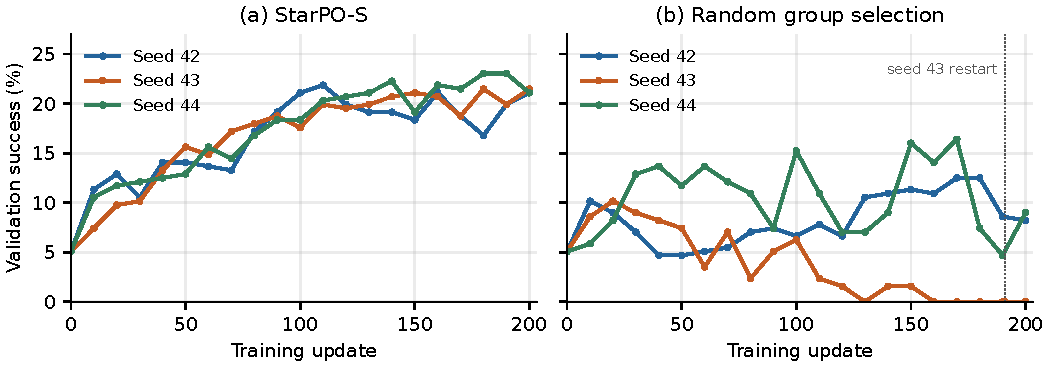
\includegraphics[width=\linewidth]{../figures/selection_curves.pdf}
\caption{Process-validation success across the three training seeds for each selection rule. All observations are shown without smoothing. The dotted line identifies the random-seed-43 restart after update 191; the update-190 comparison uses only uninterrupted histories.}\label{fig:selection}
\end{figure*}
The separation is already present before continuation. At update 190, StarPO-S solves 51, 51, and 59 of the 256 validation episodes, for 20.96\% $\pm$ 1.80 points. Random selection solves 22, 0, and 12, for 4.43\% $\pm$ 4.30 points. Figure \ref{fig:selection} shows that the final ranking is not introduced solely by the last nine updates of random seed 43. It does not establish how that run would have evolved under a fully uninterrupted RNG history.

\subsection{Two runs lose executable behavior}
At update 200, random seed 43 and no-filter seed 42 generate no parsed actions in any of their 512 test episodes. Each produces 2560 model turns with no complete answer span. Their zero task scores therefore reflect a failure to produce usable actions, rather than merely choosing valid but unsuccessful moves. Other runs retain nonzero task success.

\begin{figure*}[t]
\centering
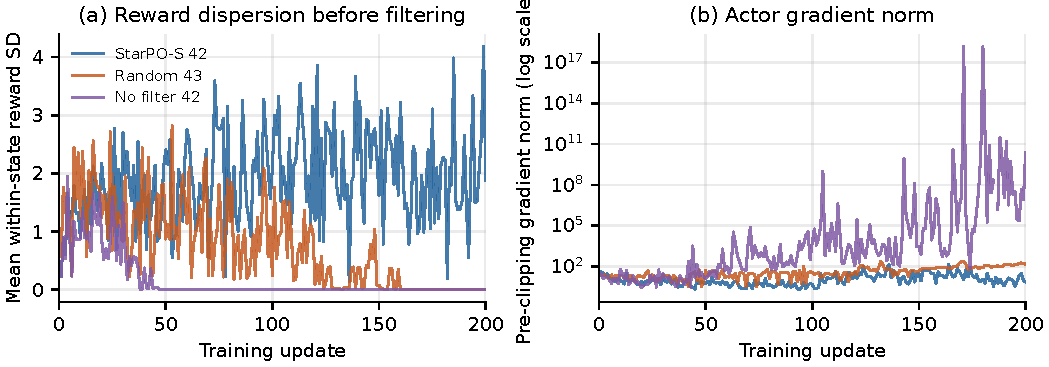
\includegraphics[width=\linewidth]{../figures/stability.pdf}
\caption{Diagnostics for the first StarPO-S run and the two zero-success runs. Left: mean within-state trajectory-score SD across all sampled groups before filtering. Right: logged actor gradient norm before clipping. The log scale displays the large excursions in the no-filter run; a nonfinite value recorded as null is left as a gap. These are associated observations, not a causal decomposition of failure.}\label{fig:stability}
\end{figure*}
Both failing runs end with zero within-state reward dispersion. Their actor gradient norms also increase, particularly in the no-filter run (Figure \ref{fig:stability}). The final logged norms are about 149 for random seed 43 and 2.43 $\times$ $10^{10}$ for no filter, compared with 7.44 for the first StarPO-S run. These norms are measured before the configured clipping operation, so a large value is not the magnitude of the applied parameter update. The joint pattern resembles instability indicators discussed in RAGEN, but our logs do not identify a unique causal mechanism or establish the full Echo Trap explanation \citep{ragen}.

\subsection{An action penalty gives mixed evidence}
The penalty run solves 112 test episodes, compared with 98 for StarPO-S at seed 42: a difference of 14 episodes, or 2.73 percentage points. Its process-validation result is slightly lower, 52 versus 54 solved episodes. More importantly for the intervention's stated purpose, its ineffective-action fraction is higher: 1320 / 3800 = 34.74\%, compared with 1254 / 4444 = 28.22\%. These fractions summarize the trajectories each policy generated, which need not visit the same states or have the same lengths. With one training seed, the experiment supports neither a reliable performance gain nor the intended reduction in wasted moves.

\subsection{Initial-board overlap does not explain the ranking}
Distinct generator seeds need not produce distinct puzzles. Comparing exact initial text grids, we find 239 unique boards among the 256 validation seeds and 486 among the 512 test seeds. Twenty board configurations occur in both sets, accounting for 22 test episodes. All eight final models receive the same seed-to-board mapping. Thus, the evaluation is held out by seed range, but not fully disjoint from validation at the board level.

A post hoc sensitivity analysis removes every test episode whose initial board matches any validation board. On the remaining 490 seed-indexed episodes, StarPO-S solves 91, 109, and 112; random selection solves 39, 0, and 25. The method ordering is unchanged. This check addresses exact validation-board overlap only. It neither deduplicates the remaining test boards nor establishes separation from every board encountered during training. Appendix \ref{app:diagnostics} gives the complete sensitivity results.

\section{Written Reasoning During Learning}\label{sec:reasoning}
\subsection{Better actions accompany shorter thoughts}
The first StarPO-S run provides a complete checkpoint-level view of text behavior. Its validation success increases from 13 / 256 (5.08\%) before training to 54 / 256 (21.09\%) at update 200. Mean words per complete thought fall from 25.07 to 3.79. Exact think-answer agreement rises from 7 / 626 complete pairs (1.12\%) to 985 / 1009 (97.62\%). Meanwhile, explicit mentions of a box, target, or wall decrease from 641 / 725 complete thoughts (88.41\%) to 0 / 1009. Figure \ref{fig:reasoning} shows the full trajectories of these measures.

\begin{figure*}[t]
\centering
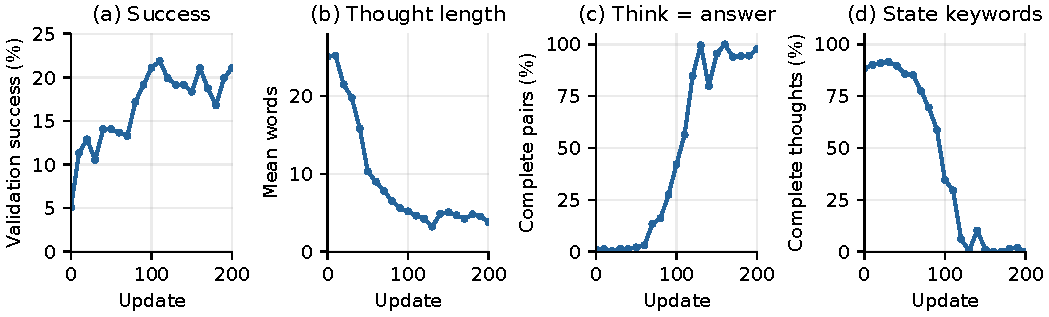
\includegraphics[width=\linewidth]{../figures/written_reasoning.pdf}
\caption{First StarPO-S run on the same 256 validation seeds at every checkpoint. Success increases while thought text shortens, thought and answer strings increasingly match, and explicit state keywords disappear. Text statistics pool turns, not episodes. Panels b and d use complete thought spans; panel c requires both complete thought and answer spans.}\label{fig:reasoning}
\end{figure*}
The change is not a monotonic loss of task performance. Validation success peaks at 56 / 256 at update 110 and remains near one fifth of the set thereafter, while agreement approaches 100\%. Across the before-and-after evaluation, 46 seeds change from failure to success and five change from success to failure. Because decoding is sampled, these transitions describe the observed episodes rather than a deterministic capability change for every puzzle.

\subsection{The final pattern repeats across training seeds}
The additional StarPO-S models show exact agreement in all complete validation pairs at update 200: 908 / 908 for seed 43 and 911 / 911 for seed 44. These denominators count turns with complete tag pairs across 256 episodes. They are not counts of levels, and they do not imply that the models solve every level.

\begin{table}[t]
\centering
\caption{Think-answer agreement in final test trajectories. Missing complete pairs make agreement undefined for the two zero-action runs. These counts use the separate 512-seed test evaluation.}\label{tab:text}
{\footnotesize
\setlength{\tabcolsep}{4pt}
\renewcommand{\arraystretch}{1.17}
\begin{tabular}{>{\raggedright\arraybackslash}p{\dimexpr 0.371681\linewidth-2\tabcolsep\relax}>{\raggedright\arraybackslash}p{\dimexpr 0.442478\linewidth-2\tabcolsep\relax}>{\raggedright\arraybackslash}p{\dimexpr 0.185841\linewidth-2\tabcolsep\relax}}
\toprule
\textbf{Method and seed} & \textbf{Matching / complete pairs} & \textbf{Agreement} \\ \midrule
StarPO-S 42 & 2021 / 2054 & 98.39\% \\
StarPO-S 43 & 1810 / 1811 & 99.94\% \\
StarPO-S 44 & 1809 / 1809 & 100.00\% \\
Random 42 & 12 / 2355 & 0.51\% \\
Random 43 & 0 / 0 & Undefined \\
Random 44 & 69 / 2096 & 3.29\% \\
Penalty 42 & 1773 / 2209 & 80.26\% \\
No filter 42 & 0 / 0 & Undefined \\
\bottomrule
\end{tabular}}
\end{table}
The same behavior is present on the test seeds (Table \ref{tab:text}). High textual agreement coexists with roughly 19-23\% task success for StarPO-S; it is therefore not equivalent to the complete behavioral failure observed in the zero-action runs. Nor does agreement mean that the model copied from an answer key: the thought appears before the answer in the generated response. The measured property is that the two fields contain identical strings.

\subsection{Two traces illustrate the distinction}
We select the lowest-numbered validation seed in each of two observed categories: failure before training followed by success at update 200, and failure at both checkpoints. This yields seeds 123 and 125. The cases illustrate the aggregate findings; they were not randomly sampled to estimate how often a particular reasoning error occurs. Their initial boards are shown in Figure \ref{fig:boards}.

\begin{figure}[t]
\centering
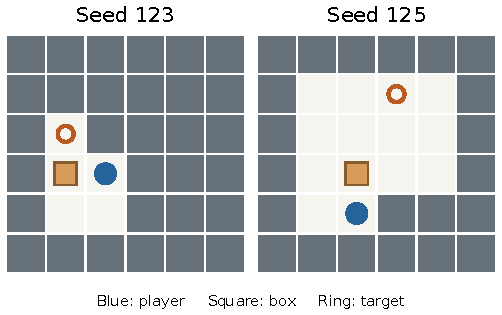
\includegraphics[width=\linewidth]{../figures/case_boards.pdf}
\caption{Initial boards for the two selected traces. Walls are gray. Both puzzles contain exactly one box and one target; the model's claim about two boxes in seed 125 is incorrect.}\label{fig:boards}
\end{figure}
On seed 123, the untrained policy begins with the thought, ``You need to push all boxes to targets. Move to the left to start the process.'' Its first action is Left, but the box cannot be pushed left through the wall. The episode fails after seven executed actions. At update 200, the policy instead produces the following two complete responses:

\begin{quote}\scriptsize\ttfamily\raggedright
<think>Right || Down</think>\\
<answer>Right || Down</answer>\\
\mbox{}\\
<think>Left || Up</think>\\
<answer>Left || Up</answer>
\end{quote}
The first Right is blocked, but Down and Left position the player below the box, and Up pushes it onto the target. The episode succeeds in four executed actions. The model gives no verbal account of this route; the thought fields duplicate the action sequences.

On seed 125, the initial policy incorrectly writes that ``there are two boxes on target,'' despite the one-box board. It then fails. At update 200, it begins with \texttt{Right || Down || Left} in both fields and still fails within the ten-action budget. Removing descriptive text therefore does not guarantee success, just as producing descriptive text does not guarantee a correct state interpretation. The saved traces permit these narrower observations without assigning an unobserved reasoning process to either policy.

\section{Discussion and Limitations}\label{sec:discussion}
The selection comparison suggests that within-state reward variation is useful for choosing update data in this setting. Groups containing different outcomes can supply learning signals that uniformly successful or uniformly unsuccessful groups lack. However, the experiment changes the group-selection rule, not reward variation independently of all other properties. Selected groups may also differ in difficulty, trajectory length, or visited states. The mechanism remains an interpretation of the observed method comparison.

The text results identify a second issue that success rate alone would miss. Task return does not directly reward a correct description of a box, a wall, or an intended route. A policy can therefore improve its action choices while making its explicit thought field largely redundant with its answer. The disappearance of state words strengthens the description of this output change, but the keyword list is coarse and short text can still encode a useful plan. We make no claim that internal computation has stopped or that verbosity is desirable in itself.

The two forms of degradation should also remain separate. Short, repeated thought text appears in models that still act and solve puzzles. Empty or malformed answers appear in the two zero-success models and prevent execution. A single label such as reasoning collapse would obscure this behavioral difference. Monitoring action parsing, task success, and text structure separately is more informative than using any one of them as a proxy for the others.

The evidence is limited to one small instruction-tuned model and one short-horizon puzzle environment. Three training seeds are available only for the main selection comparison. The penalty and no-filter variants each have one seed, and no filter changes update data volume. The seed settings vary driver and environment randomness while leaving historical veRL and vLLM internal defaults unchanged. Two runs are continuations with reset driver state. Evaluation uses one sampled rollout per seed, and the initial-board audit shows that seed separation is weaker than layout separation. These restrictions preclude broad claims about larger agents or reliable performance improvements.

Further experiments should first use more training seeds, repeated evaluation decodes, and board-disjoint splits. Equal-token or equal-time comparisons would clarify the cost of selection. Testing assistant-only loss masking would isolate an inherited implementation choice. To study whether written reasoning contributes to action quality, one could intervene on the thought field while holding the board and action budget fixed, rather than simply reward longer text. None of these interventions is part of the present evidence.

\section{Conclusion}\label{sec:conclusion}
In this Sokoban study, StarPO-S produces better task performance than random group selection across the tested seeds, but its explicit thoughts become shorter and nearly identical to its answers. Failure diagnostics reveal a distinct outcome in two comparison runs: loss of executable actions accompanied by zero reward dispersion and large gradient norms. The action-penalty experiment remains inconclusive. Together, these observations show why task success, training stability, and written reasoning should be measured separately when assessing multi-turn reinforcement learning.

\newpage
\bibliographystyle{plainnat}
\bibliography{references}
\onecolumn
\appendix
\section{Implementation and Reproduction Details}\label{app:reproduction}
The experiments used one NVIDIA H100 80 GB GPU, eight allocated CPU cores, and 64 GB of host memory. The observed software stack included Python 3.10, PyTorch 2.6.0 with CUDA 12.4, Transformers 4.49.0, and vLLM 0.8.2. RAGEN was pinned to commit {\scriptsize\texttt{f92df5d67266af273d9c5ea4d25eb96d235b41ff}}; the nested veRL source was pinned to {\scriptsize\texttt{797f9994b73f6335aa2349cdb2e9bb2a42f13f5c}}. The Qwen2.5-0.5B-Instruct checkpoint revision was {\scriptsize\texttt{7ae557604adf67be50417f59c2c2f167def9a775}}. The public source snapshot records the small experiment-specific modifications separately from the upstream files.

\begin{statictable}
\centering
\caption{Shared settings for the completed runs. Penalty and no-filter changes are described in Section \ref{sec:design}. An update denotes one outer rollout-and-optimization iteration, not one gradient mini-batch.}\label{tab:config}
{\small
\setlength{\tabcolsep}{4pt}
\renewcommand{\arraystretch}{1.17}
\begin{tabular}{>{\raggedright\arraybackslash}p{\dimexpr 0.276423\linewidth-2\tabcolsep\relax}>{\raggedright\arraybackslash}p{\dimexpr 0.195122\linewidth-2\tabcolsep\relax}>{\raggedright\arraybackslash}p{\dimexpr 0.268293\linewidth-2\tabcolsep\relax}>{\raggedright\arraybackslash}p{\dimexpr 0.260163\linewidth-2\tabcolsep\relax}}
\toprule
\textbf{Setting} & \textbf{Value} & \textbf{Setting} & \textbf{Value} \\ \midrule
Board / box count & 6 $\times$ 6 / 1 & Target updates & 200 \\
Model turns / actions & 5 / 10 & Actions per turn & At most 5 \\
Groups $\times$ episodes & 8 $\times$ 16 & Retained episodes & 32; no filter 128 \\
Train / eval temperature & 1.0 / 0.5 & New tokens per turn & At most 400 \\
Actor / critic LR & $10^{-6}$ / $10^{-5}$ & PPO epochs & 1 \\
Mini / micro batch & 32 / 4 & Discount / GAE lambda & 1.0 / 1.0 \\
PPO ratio interval & [0.80, 1.28] & Entropy / KL coefficient & 0.001 / 0 \\
Actor / critic grad clip & 1.0 / 1.0 & Reward normalization & Identity \\
Response-only mask & Disabled & Per-turn score mode & Disabled \\
\bottomrule
\end{tabular}}
\end{statictable}
The initial allocation lasted 51 minutes 5 seconds and contained a three-update smoke test followed by a fresh 200-update StarPO-S seed-42 run. The follow-up allocation lasted 7 hours 53 minutes 10 seconds and trained seven further models; two stopped early under soft time budgets. An evaluation import error from a missing context-manager source file ended that batch after training. The source was restored, and a third allocation of 1 hour 42 minutes 17 seconds evaluated the available checkpoints, completed the two interrupted runs, and evaluated their final checkpoints. Total allocation time was approximately 10.44 GPU-hours, including startup, evaluation, and checkpointing.

The repository retains ten test evaluation records: eight final update-200 evaluations and two earlier evaluations of incomplete checkpoints. Only the eight final evaluations contribute to the main table. Raw compressed logs are hash-checked, and the analysis merges continuation histories without double-counting their restart checkpoint. The missing-file execution issue is distinct from the model failures: subsequent evaluations completed successfully and still found no parsed actions for the two zero-success models.

The data can be audited without a GPU using \texttt{python scripts/analyze.py --verify}, followed by \texttt{python scripts/plot.py}, from the repository root. Recorded configurations and commands for model download, smoke testing, training, evaluation, and resumption are in \texttt{docs/reproduction.md}. The training launcher and reconstructed dependency recipe were packaged after the experiments; their CPU configuration checks and analysis have been tested, but the public packaging has not been rerun end to end in a fresh GPU installation. Model weights and optimizer checkpoints are not distributed with the repository.

\clearpage
\section{Additional Diagnostics}\label{app:diagnostics}
\subsection{Loss and return curves}
\begin{staticfigure}
\centering
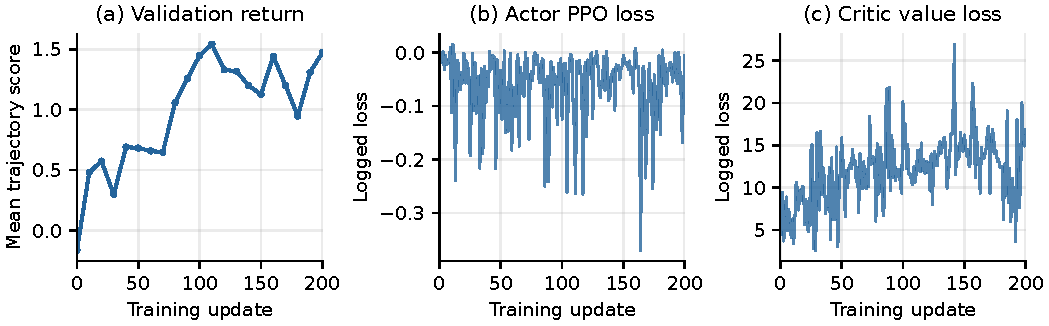
\includegraphics[width=\linewidth]{../figures/loss_and_return.pdf}
\caption{Unsmoothed validation trajectory score and training losses for StarPO-S seed 42. The PPO actor loss and critic value loss are optimization diagnostics on changing rollout data; neither is an accuracy measure or expected to decrease monotonically. Validation score includes the shared format penalty and is distinct from binary task success.}\label{fig:loss}
\end{staticfigure}
For the first StarPO-S run, mean validation trajectory score increases from -0.1656 to 1.4719 (Figure \ref{fig:loss}). The process-validation success rate increases over the same interval, but the intermediate peaks do not define a selected final model: all reported final comparisons use update 200.

\subsection{Sensitivity to validation-board overlap}
\begin{statictable}
\centering
\caption{Post hoc test sensitivity after removing the 22 seed-indexed episodes with an initial board also present in validation. The retained 490 episodes contain 466 distinct initial text grids. Remaining duplicates are retained with their original seed weights.}\label{tab:sensitivity}
{\small
\setlength{\tabcolsep}{4pt}
\renewcommand{\arraystretch}{1.17}
\begin{tabular}{>{\raggedright\arraybackslash}p{\dimexpr 0.446429\linewidth-2\tabcolsep\relax}>{\raggedright\arraybackslash}p{\dimexpr 0.303571\linewidth-2\tabcolsep\relax}>{\raggedright\arraybackslash}p{\dimexpr 0.250000\linewidth-2\tabcolsep\relax}}
\toprule
\textbf{Method and seed} & \textbf{Solved / 490} & \textbf{Success} \\ \midrule
StarPO-S 42 & 91 & 18.57\% \\
StarPO-S 43 & 109 & 22.24\% \\
StarPO-S 44 & 112 & 22.86\% \\
Random 42 & 39 & 7.96\% \\
Random 43 & 0 & 0.00\% \\
Random 44 & 25 & 5.10\% \\
Penalty 42 & 108 & 22.04\% \\
No filter 42 & 0 & 0.00\% \\
\bottomrule
\end{tabular}}
\end{statictable}
Board matching uses exact equality of the initial text grid, including the player, box, target, and walls. Rotations and reflections are not merged. The audit compares the initial board for every test seed across all eight final models and confirms identical mappings. This check is narrower than proving that the evaluation contains novel layouts relative to the full training history.

\subsection{Sequence length and incomplete outputs}
The historical metric \texttt{response\_length/mean} measures the serialized training sequence, including prompts and environment feedback, because the context manager exposes almost the full input sequence as its response tensor. It should not be labeled as newly generated answer length. In contrast, \texttt{train/response\_length} uses the assistant-segment mask, including chat-format tokens and processed responses. Over the last 20 updates, their means are respectively 580.30 and 98.76 tokens for StarPO-S seed 42, 2438.27 and 1829.00 for random seed 43, and 2624.85 and 2038.74 for no filter. The word-count analysis in Section \ref{sec:reasoning} avoids interpreting either token metric as a measure of reasoning quality.

At the first validation checkpoint there are 725 complete thought spans but only 626 complete thought-answer pairs. At update 200 there are 1009 of each. This difference explains why length and keyword statistics have a different initial denominator from the agreement statistic. For the two failed final models, no complete answer pairs are available; reporting 0\% agreement would conflate missing structured output with disagreement between two observed strings.

\end{document}
